\chapter{Results} 
\label{chap:results}
%\begin{enumerate}
%\item all data
%\item analysis done
%\item discussions
%\item comparisons
%\end{enumerate}

\begin{figure}
  \begin{center}
    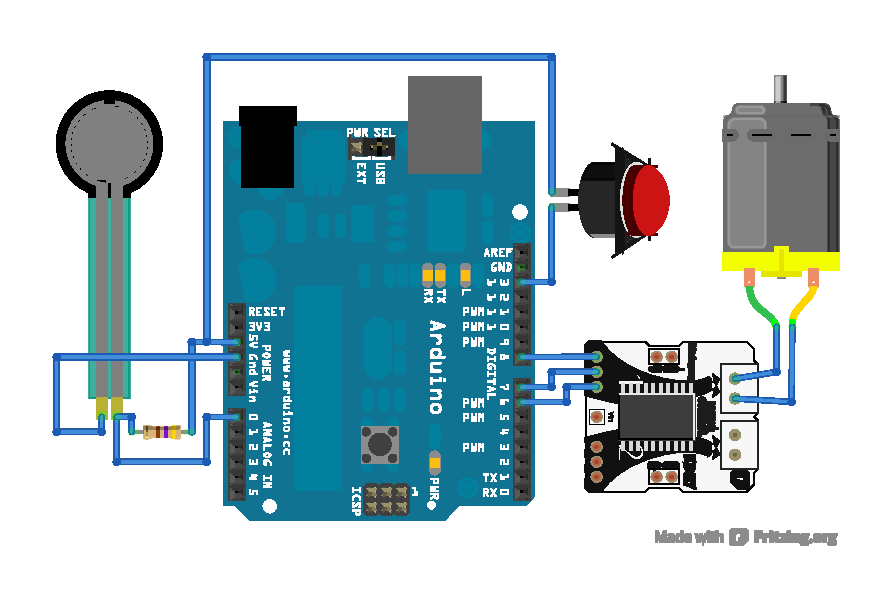
\includegraphics[width=1.0\columnwidth]{Figures/simple-example.pdf}
    \caption{The components of a simple single-board \xten setup} \label{fig:singleboard}
  \end{center}
\end{figure}

This chapter presents evidence showing how the \xten architecture achieves its objectives through the hardware and software platform. We demonstrate this by applying the framework across a number of practical examples before discussing the outcomes.

 We demonstrate the framework in action by showing excerpts of sample programs for a simple mobile robot with a number of sensors and actuators distributed across one or more daughterboards. These examples demonstrated the how modularity, scalability and extensibility are expressed through code and hardware configuration.
 
All tests and examples were done using the Arduino Prototyping system since this was the chosen platform used to prototype the \xten architecture. The fundamental concepts however were general enough to be implemented on any modern mirocontroller.

Listing~\textbf{\ref{code:example}} is a typical code setup for a very simple mobile robot illustrated in Figure \textbf{\ref{fig:singleboard}}. All the sensors and actuators were placed on one board; for this particular implementation, we utilised the \textbf{internal} daughterboard which is hosted on the same board as the motherboard. This robot has one actuator (a DC motor connected to an external H-bridge), a force sensor and a pushbutton sensor.


%\begin{multicols}{2}
	\begin{listing}
		\footnotesize
		\begin{minted}[bgcolor=bg,baselinestretch=1,frame=lines,framesep=2mm,label={\xten Sample code}]{c}

/**
* Import the necessary libraries for the motherboard, 
* internal daughterboard and the peripheral bus
**/
#include <Wire.h>  
#include <X10ABOT_MB.h>
#include <X10ABOT_DB.h> //Include the internal daughterboard #0 (SELF)

//Initialise the DC motor on daughterboard #0 (SELF), actuator port #1
Actuator motor1(SELF,1);
//Initialise force sensor on daughterboard #0 (SELF), sensor port #1
Sensor force1(SELF,1);
//Initialise force sensor on daughterboard #0 (SELF), sensor port #2
Sensor pushbutton(SELF,1);

void setup(){}
void loop(){
//Continuously check the sensors for a reading
  if(pushbutton.readDigitalB() || (force1.readAnalog()>100)){
    motor1.aB(); //Turn motor1 on by sending LO on pin a and HI on pin B
    motor1.pwm_a(100); //operate motor1 at full power (100%) 
  }else{
    motor1.ab();//Turn motor1 off by sending LO on pin a and pin b
  }
}	 
	\end{minted}
		\caption{Example of the \xten architecture on a simple - single board robot.} \label{code:example}
	\end{listing}
%	\vfill
%	\columnbreak



Listing~\textbf{\ref{code:example}} is a simple program that drives the motor at full speed if either the touch sensor records an input or if there is a force on the force sensor above a certain threshold, otherwise the motor will be given the off signal.

%\end{multicols}
In this instance, there are two types of devices that are declared, \textbf{Sensor} and \textbf{Actuator}. These represent the parent classes of all sensors and actuators respectively in the \xten architecture. This example utilises the parent class but for more complex sensors and actuators, a subclass would have been appropriate. All other sensor and actuator sub-types inherit from these two classes of devices, overriding where necessary.

It should be noted that it was necessary to include the library for both the motherboard and the daughterboard since they share the same Arduino board. Daughterboard address \#0 or the constant \textbf{SELF} is reserved for the internal daughterboard on the same physical Arduino platform.

	\section{Modularity} % (fold)
	\label{sec:modularity}
% section modularity (end)
Adding an extra capability was easily and seamlessly carried out using the \xten architecture. We included an extra daughterboard that represented a complete subsystem using sensors and actuators. In our example in Figure \textbf{\ref{fig:modularity}}, an extra DC motor and a light sensor were added as a single module. The \xten architecture allowed for this new addition as a daughterboard via the peripheral bus. The module was just as easily added in software. The daughterboard was assigned a unique arbitrary address of \textbf{\#9}. Instructions were then added to activate the new DC motor if there was light intensity above a certain threshold on the sensor. We could have easily controlled the existing motor or mixed the logic between the existing components, however for clarity we made it so that the modules would operate independently.  In the Listing~\ref{code:modularity}, we demonstrate how we added this extra functionality.

\begin{figure}[h!]
  \begin{center}
    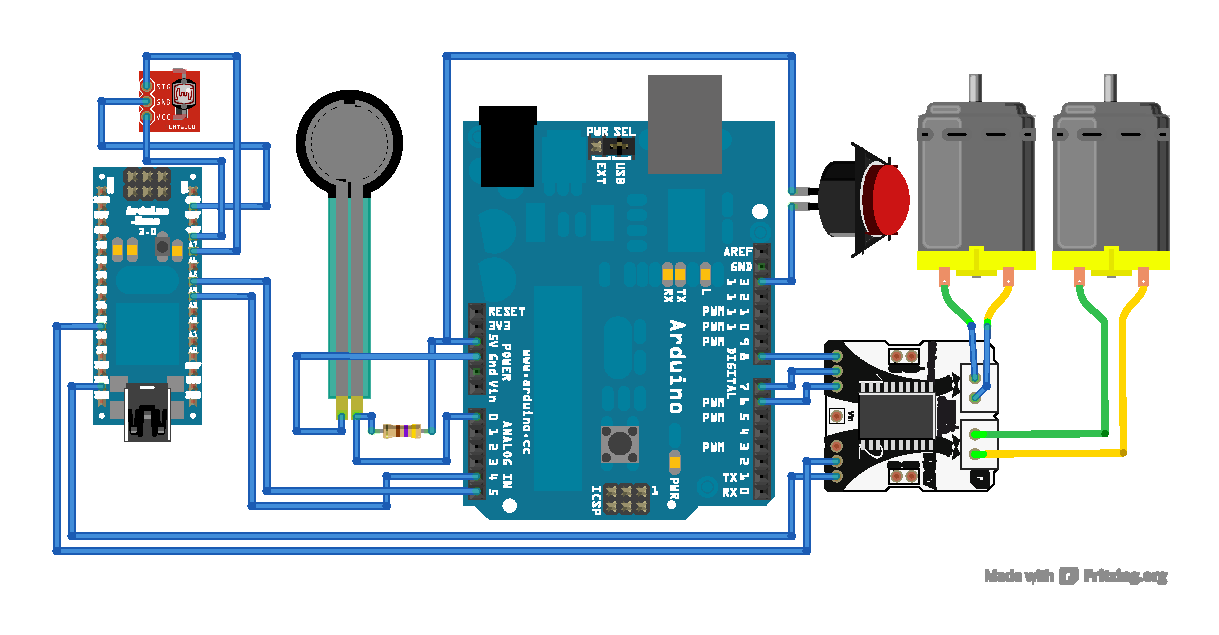
\includegraphics[width=1.0\columnwidth]{Figures/modular-example.pdf}
    \caption{The components of a Modular single-board \xten Example}\label{fig:modularity}
  \end{center}
\end{figure}

\begin{listing}
		\footnotesize
		\caption{Example of code modularity (the code components were separated to emphasise modularity).} \label{code:modularity}
		\begin{minted}[bgcolor=bg,baselinestretch=1,frame=lines,framesep=2mm,label={Modularity in Code}]{c}
        \end{minted}
        \begin{minted}[bgcolor=bg,baselinestretch=1]{c}
/**
* Import the necessary libraries for the motherboard, 
* internal daughterboard and the peripheral bus
**/
#include <Wire.h>  
#include <X10ABOT_MB.h>
#include <X10ABOT_DB.h> //Include the internal daughterboard #0 (SELF)

//Initialise the DC motor on daughterboard #0 (SELF), actuator port #1
Actuator motor1(SELF,1);
//Initialise force sensor on daughterboard #0 (SELF), sensor port #1
Sensor force1(SELF,1);
//Initialise force sensor on daughterboard #0 (SELF), sensor port #2
Sensor pushbutton(SELF,1);
   
void setup(){}
void loop(){
//Continuously check the sensors for a reading
if(pushbutton.readDigitalB() || (force1.readAnalog()>100)){
    motor1.aB(); //Turn motor1 on by sending LO on pin a and HI on pin B
    motor1.pwm_a(100); //operate motor1 at full power (100%) 
  }else{
    motor1.ab();//Turn motor1 off by sending LO on pin a and pin b
  }
 \end{minted}
 \begin{minted}[bgcolor=hilite,baselinestretch=1]{c}
 const byte BOARD2 = 9; //Constant with arbitrary daughterboard address
 //Declare motor on daughterboard #9, actuator port #1
 Actuator motor2(BOARD2,1);
 //Declare force sensor on daughterboard #9, sensor port #1
 Sensor lightSensor(BOARD2,1);
 
//Added extra functionality with a new sensor and a new actuator
//on daughterboard #9 while light is on the sensor, activate motor2
if (lightSensor.readAnalog()>700)
  {
    motor2.Ab(); //Turn motor2 on by sending HI on pin A and LO on pin b
    motor2.pwm_a(50); //operate motor2 at half power (50%)
  }else{
    motor2.ab();//Turn motor1 off by sending LO on pin a and pin b
  }
}	 
	\end{minted}
		
\end{listing}
In the code example at Listing \ref{code:modularity}, even with the addition of two independent devices, \emph{motor1} and \emph{lightSensor} to the system, it did not affect the existing code but fit seamlessly in the development process. Separate code was added to carry out their operation which never needed to interact with the existing system. There needed to be no special accommodation for the new module in the existing code. There was no significant modification made to the existing hardware setup even with the fact that an extra physical component, another daughterboard, was added to the system. The \xten design allowed a pluggable interface that facilitated adding new code and hardware with minimal modification to the existing setup.
All these features are an indication of a truly modular architecture. As previously defined, we included an entire subsystem without modifying the existing components. The modules can be removed just as easy as they were installed. The level of expertise, with regard to specialised knowledge required to modify this system is also relatively minimal when compared to a generic prototyping platform like the Arduino due to the abstraction in its design.


% chapter findings_and_results (end)
\section{Extensibility and Abstraction} % (fold)
\label{sec:extensibility_abstraction}
We demonstrate the \xten architecture's ability to support new and varied types of sensors and actuators. This is accomplished by creating a subclass to either of the existing Sensor or Actuator classes. These parent classes support all the generic operations on all the available sensor and actuator ports. By creating a subclass, all the parent class properties and functions will be inherited. Devices with unique configurations can be supported by utilising the same abstracted daughterboard access available to the parent classes requiring no knowledge of the low-level details of the hardware.
In the following example, we will define a simple, yet complete library that reads and interprets the data from a thermistor temperature sensor. The raw analog value will be read then we will apply some computations to acquire a useful output. The class will support functions that return temperature values in both celsius and fahrenheit units. This code was sourced from the Arduino Playground \parencite{therm} as a simple example to acquire thermistor temperature readings. We made a few simple modification that allowed the same code to be applicable to the \xten architecture.
\begin{listing}
		\footnotesize
		\caption{Example: A complete library for a thermistor temperature sensor.} \label{code:therm}
		\begin{minted}[bgcolor=bg,baselinestretch=1,frame=lines,framesep=2mm,label={Thermistor Library}]{c}
#include "../X10ABOT_MB.h"
#include <math.h>
class Thermistor: public Sensor
{
  private:
    byte _db, _port;
  public:
    Thermistor(byte db_address, byte port_number):Sensor(_db, _port){
      _db = db_address;
      _port = port_number;
    }
    ~Thermistor(){};
    double readThermistorCelsius() {
    \end{minted}
    \begin{minted}[bgcolor=hilite,baselinestretch=1]{c}
        //The analog microcode requests the raw sensor value
        int RawADC = analog(_db,_port); 
    \end{minted}
    \begin{minted}[bgcolor=bg,baselinestretch=1]{c}
        double Temp;
        Temp = log(((10240000/RawADC) - 10000));
        Temp = 1/(0.001129148+(0.000234125+(0.0000000876741*Temp*Temp))*Temp);
        Temp = Temp - 273.15;            // Convert Kelvin to Celsius
        return Temp;
    }
    double readThermistorFarenheit() {
    // Convert Celsius to Fahrenheit
        return (readThermistorCelsius()* 9.0)/ 5.0 + 32.0;
    }
};
	\end{minted}
		
\end{listing}

The conversion component of the library in Listing \ref{code:therm} is an almost exact replica of the fragment of code extracted from the Arduino library. In the \textbf{readThermistorCelsius} function, the main change (highlighted in yellow) can be found where the code accesses the analogue pin to read the raw data value acquired from the sensor. The \xten framework possesses special functions that access hardware components. For this particular case, the \textbf{analog(\_db,\_port)} function was invoked, access to this function was inherited by extending the Sensor class. This is a method used to abstract the analog pin on the sensor port so it becomes hardware independent. The analogue pin belongs on a daughterboard \textbf{\_db} on a particular sensor port \textbf{\_port}. The raw analogue value is then returned to the calling function where it is further processed.

This thermistor library can then be easily utilised by the user as follows:

The code in Listing~\ref{code:thermcode} presents a temperature monitoring system that watches the temperature that it receives from two thermistors. If the value read from the thermistors goes beyond particular thresholds for either of them, an alarm is triggered.
\begin{listing}
		\footnotesize
		\caption{Example application of the thermistor temperature sensor library.} \label{code:thermcode}
		\begin{minted}[bgcolor=bg,frame=lines,baselinestretch=1,framesep=2mm,label={Thermistor Example Application}]{c}
#include <Wire.h>  
#include "x10sions/Thermistor.h"
#include <X10ABOT_MB.h>
const byte FREEZER = 17; //Create a constant with the daughterboard address
const byte OVEN = 108;
const byte CONTROL_BOARD = 10;

//Declare thermistor on daughterboard #17, sensor port #1
Thermistor coldSensor(FREEZER,1);
//Declare thermistor on daughterboard #108, sensor port #6
Thermistor hotSensor(OVEN,6);
//Declare digital alarm on daughterboard #10, actuator port #3
Actuator alarm(CONTROL_BOARD,3,A);

void setup(){}
void loop(){
//Continuously check the sensors to see if temperature within threshold
  if((coldSensor.readThermistorCelsius() > 1 )
      || hotSensor.readThermistorFarenheit()<200){
  alarm.on_a(); //Turn on alarm 
  }
}
	\end{minted}
		
\end{listing}

A typical end user would not be involved in creating libraries for sensors. They would have only been exposed to the setup in Listing~\ref{code:thermcode}. The only requisite knowledge would be familiarity with the supported list of functions specified for a thermistor. In this case only \textbf{readThermistorFarenheit()} and  \textbf{readThermistorCelsius()} are specified and both have been used.
The library for a thermistor was included and it became very straightforward to utilise the sensor readings afterwards.
% section extensibility and abstraction (end)

\section{Scalability} % (fold)
\label{sec:scalability}

% section scalability (end)
Based on the results gathered from testing for modularity, an inherent property for scalability can be observed. The method of modular addition lends itself to be scalable to tens of modules as defined by the specifications of the peripheral bus protocol. Scalability is not only measured by how many devices can be connected to the system, but we must take into consideration the performace of the system when all these devices are operational. We therefore need to benchmark the performance of the architecture implemented on the Arduino platform. This is necessary to evaluate what type of applications will be suitable for executions based on the speed at which instructions are excuted. This can determine how the system will perform when under duress from multiple hardware devices simultaneously executing instructions and requesting attention. These statistics can then be evaluated to deduce the architecture's suitability for a particular project and at what point would it become unusable. When operating with daughterboards acrooss the peripheral bus, the \xten architecture's major limiting factor becomes the speed of data transfer. The default speed of the peripheral bus when using the Arduino plaftorm is 100Kb/s, this can be further configured to go as high as 400Kb/s. For our application on the Arduino we had best result when performing at approximately 300Kb/s. We performed a number of tests to determine the latency of each type of basic instruction to see how they would affect the performance of the entire system. All tests below were carried out on the Arduino Mega, using the Atmel \texttrademark ATMega1280 microcontroller.

We carried out a few timing tests to evaluate the performance of the \xten framework on the Arduino platform. The tests were done using one motherboard and three daughterboards. The typical robotics project may never require as many daughter boards since one Arduino Mega may support up to eight sensor ports and six actuator ports. The smaller Arduino Uno can support up to three sensor ports and two actuator ports. Any combination of one or more of these Arduino boards can be used to implement the \xten architecture.
We did timing tests to measure the latency between the command request and the response. We also ran tests to see if there was any measurable difference when the peripheral bus is congested with a rapid succession of events for all the three daughterboards.

The sample below displays the result of our timing experiment, the timing utility on the Arduino has a maximum resolution of 4 micro second intervals.
%Table \ref{table:onboard} presents 


The Sample Standard Deviation $$s = \sqrt{\frac{1}{N-1} \sum_{i=1}^N (x_i - \overline{x})^2}$$

Direct Arduino Board readings

The Sample digitalOut: %[12, 12, 16, 16, 12, 12, 12, 16, 16, 12, 12, 16, 16, 12, 12, 12, 16, 16, 12, 12]
average = 13.6
s = 2.01

The Sample digitalIn: %[20, 16, 16, 16, 16, 12, 16, 16, 12, 16, 16, 12, 16, 16, 12, 16, 16, 20, 16, 16]
average = 15.6
s = 2.21

The Sample pwm: %[12, 12, 12, 12, 12, 12, 12, 12, 12, 12, 12, 12, 12, 12, 12, 12, 12, 16, 12, 12]
average = 12.2
s = 0.89

The Sample analogue:%[112, 120, 116, 116, 116, 124, 112, 112, 112, 120, 116, 116, 116, 116, 112, 112, 112, 120, 116, 116]
average = 115.6
s = 3.41

Onboard readings

The Sample digitalOut:% [40, 40, 36, 40, 40, 40, 40, 40, 36, 40, 40, 40, 40, 40, 36, 40, 40, 40, 40, 40]
average = 39.4
s = 2.15

The Sample digitalIn:% [84, 88, 84, 84, 84, 84, 84, 80, 84, 80, 88, 84, 84, 84, 80, 84, 84, 80, 84]
average = 83.58
s = 2.27

The Sample pwm:% [60, 56, 56, 56, 60, 60, 56, 56, 60, 60, 56, 56, 56, 60, 60, 56, 56, 60, 60, 56]
average = 57.8
s = 4.17

The Sample analogue:% [212, 216, 212, 216, 212, 212, 212, 216, 216, 216, 216, 216, 216, 216, 220, 216, 216, 224, 216215.58]
average = 215.58
s = 2.95

Offboard readings

The Sample digitalOut:% [260, 268, 260, 260, 260, 260, 260, 260, 268, 260, 264, 260, 260, 260, 260, 268, 260, 260, 260, 260]
average = 261.4
s = 2.98

The Sample digitalIn:% [556, 556, 556, 552, 556, 552, 560, 556, 552, 552, 556, 552, 556, 560, 556, 552, 552, 556, 552, 556]
average = 554.8
s = 2.63

The Sample pwm :%[320, 316, 320, 320, 320, 320, 320, 316, 320, 324, 316, 320, 320, 316, 320, 316, 320, 316, 320, 320]
average = 319
s = 2.20

The Sample analogue:% [668, 656, 668, 656, 656, 660, 656, 664, 656, 656, 656, 656, 652, 656, 656, 656, 656, 652, 672, 656]
average = 658.2
s = 5.43
\begin{table}[h!]
    %\scriptsize {
	%\centering
	\caption{Table showing microcode latency in microseconds($\mu$s) on the on-board daughterboard for over 20 consecutive executions.}\label{table:onboard}
	\begin{tabular}{|l|l|l|l|}
	\toprule
 \multicolumn{4}{c}{\textbf{ONBOARD daughterboard}} \\\hline

digitalOut & digitalIn & pwm & analogue \\\hline
40 & 50084 & 60 & 50212\\\hline
40 & 50088 & 60 & 50216 \\\hline
40 & 50084 & 60 & 50212 \\\hline
36 & 50084 & 60 & 50216 \\\hline
40 & 50084 & 56 & 50212 \\\hline
40 & 50084 & 60 & 50212 \\\hline
40 & 50084 & 60 & 50212 \\\hline
40 & 50080 & 60 & 50216 \\\hline
40 & 50084 & 60 & 50216 \\\hline
48 & 50080 & 56 & 50216 \\\hline
40 & 50088 & 56 & 50216 \\\hline
40 & 50084 & 56 & 50216 \\\hline
40 & 50084 & 60 & 50216 \\\hline
36 & 50084 & 60 & 50216 \\\hline
40 & 50080 & 60 & 50220 \\\hline
40 & 50084 & 64 & 50216 \\\hline
40 & 50084 & 56 & 50216 \\\hline
40 & 50080 & 60 & 50224 \\\hline
40 & 50084 & 56 & 50216 \\\hline
\multicolumn{4}{c}{Average Times} \\\hline
40.00 & 50083.58 & 58.95 & 50215.58

%}
\end{tabular}
\end{table}

The latency for output operations took significantly less time than that of input operations. This was expected since there is no waiting period to request the value of the data from the port on the daughterboard for output operations. Conversely with input operations, the system was programmed with a set delay of \_\_\_\_\_\_ which was necessary to allow for the sensors to return their values.

\begin{table}
    %\scriptsize {%
	\centering
	\caption{Table showing microcode latency in microseconds($\mu$s) on the off-board daughteroard over 20 consecutive executions.}
	
	\begin{tabular}{|l|l|l|l|}
	\toprule
 \multicolumn{4}{c}{\textbf{OFFBOARD daughterboard}} \\\hline
digitalOut & digitalIn & pwm & analogue\\\hline
568 & 51320 & 688 & 51328\\\hline
560 & 51320 & 684 & 51320\\\hline
568 & 51324 & 684 & 51324\\\hline
568 & 51324 & 684 & 51328\\\hline
568 & 51332 & 684 & 51324\\\hline
564 & 51324 & 684 & 51332\\\hline
564 & 51324 & 684 & 51328\\\hline
564 & 51320 & 688 & 51324\\\hline
564 & 51320 & 680 & 51332\\\hline
568 & 51324 & 688 & 51324\\\hline
564 & 51324 & 680 & 51324\\\hline
568 & 51324 & 684 & 51324\\\hline
564 & 51320 & 684 & 51328\\\hline
568 & 51328 & 684 & 51324\\\hline
560 & 51320 & 688 & 51328\\\hline
564 & 51320 & 688 & 51328\\\hline
568 & 51324 & 684 & 51332\\\hline
564 & 51320 & 684 & 51324\\\hline
564 & 51320 & 684 & 51324\\\hline
\multicolumn{4}{c}{Average Times} \\\hline
565.26 & 51322.74 & 684.63 & 51326.32

%}
\end{tabular}
\end{table}

We carried out an experiment to determine how the system performed when executing a barrage of instruction and obtained the results listed in table X below. 
\begin{table}
    %\scriptsize {%
	\centering
	\caption{Table showing microcode latency in microseconds($\mu$s) on the off-board daughteroard for number of instructions executed(no.) and associated time it took to complete over 5050 consecutive executions of digitalOut.}
	
	\begin{tabular}{|l|l||l|l||l|l||l|l||l|l||}
	\toprule
 \multicolumn{10}{c}{\textbf{OFFBOARD daughterboard barrage}} \\\hline


no. & time ($\mu$s)& no. & time ($\mu$s)& no. & time ($\mu$s)& no. & time ($\mu$s)& no. & time ($\mu$s) \\\hline
1 & 568 & 21 & 11840 & 41 & 23120 & 61 & 34380 & 81 & 45648 \\\hline
2 & 1132 & 22 & 12412 & 42 & 23676 & 62 & 34936 & 82 & 46216 \\\hline
3 & 1696 & 23 & 12972 & 43 & 24244 & 63 & 35516 & 83 & 46780 \\\hline
4 & 2268 & 24 & 13524 & 44 & 24796 & 64 & 36080 & 84 & 47352 \\\hline
5 & 2820 & 25 & 14108 & 45 & 25364 & 65 & 36620 & 85 & 47916 \\\hline
6 & 3384 & 26 & 14656 & 46 & 25932 & 66 & 37208 & 86 & 48480 \\\hline
7 & 3948 & 27 & 15228 & 47 & 26484 & 67 & 37772 & 87 & 49044 \\\hline
8 & 4520 & 28 & 15788 & 48 & 27068 & 68 & 38332 & 88 & 49600 \\\hline
9 & 5072 & 29 & 16352 & 49 & 27620 & 69 & 38880 & 89 & 50172 \\\hline
10 & 5636 & 30 & 16908 & 50 & 28188 & 70 & 39456 & 90 & 50736 \\\hline
11 & 6212 & 31 & 17472 & 51 & 28760 & 71 & 40028 & 91 & 51296 \\\hline
12 & 6768 & 32 & 18044 & 52 & 29316 & 72 & 40588 & 92 & 51860 \\\hline
13 & 7332 & 33 & 18600 & 53 & 29872 & 73 & 41156 & 93 & 52420 \\\hline
14 & 7896 & 34 & 19172 & 54 & 30452 & 74 & 41696 & 94 & 52980 \\\hline
15 & 8460 & 35 & 19732 & 55 & 31008 & 75 & 42276 & 95 & 53552 \\\hline
16 & 9020 & 36 & 20300 & 56 & 31552 & 76 & 42844 & 96 & 54112 \\\hline
17 & 9584 & 37 & 20856 & 57 & 32140 & 77 & 43408 & 97 & 54672 \\\hline
18 & 10148 & 38 & 21424 & 58 & 32696 & 78 & 43976 & 98 & 55244 \\\hline
19 & 10708 & 39 & 21988 & 59 & 33248 & 79 & 44536 & 99 & 55804 \\\hline
20 & 11280 & 40 & 22548 & 60 & 33828 & 80 & 45096 & 100 & 56364 \\\hline
\multicolumn{10}{c}{Total time taken: 2847984} \\\hline
\end{tabular}
\end{table}
 The results showed that even at high instruction thoroughput, the time to execute a particular instruction does not vary significantly from its latency as a single instruction.


\section{Discussion} % (fold)
\label{sec:Discussion}

 however, other hardware specific limitations may come into play. These may include, clock speed and available RAM, all of which may differ, even across Arduino hardware platforms.

% section economy (end)
